\section{Implementation}

\begin{figure}[H]
\centering
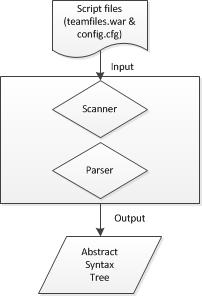
\includegraphics[scale=1]{rapport/6/figures/parser}
\label{fig:parser}
\caption{Parser}
\end{figure}

\subsubsection{Getting the data}
Inside the simulator figure \ref{fig:simulator} we implemented a \textit{GameDataRetriever} class which retrieves data from the Decorated Abstract Syntax Tree[DAST], so we have reused the visitor pattern to run through the tree and collect all the data needed to run the simulator. The \textit{GameDataRetriever} saves the data in the GameClasses which contains Regiment, Grid, Team and Tile- classes. These classes contains all the useful data for the simulator to run.
\subsubsection{Validating the data}
After all the data have been retrieved from the DAST we have to validate if the data is correct. By correct we mean that e.g. in the config.cfg file a \textit{Maxima} is present, and if the teamfiles.war contains larger numbers than the \textit{Maxima} requires, there will be an error. The config.cfg file contains standards for which the programmers teamfiles.war will be assigned to if they haven't assigned their own constants. An example: if the teamfile.war does contain a regiment with some size and a name of the regiment, but nothing more, the regiment will then be assigned the default/standard values, if the standard values is nowhere to be found in the config.cfg file there will be an error as well.

\begin{figure}[H]
\centering
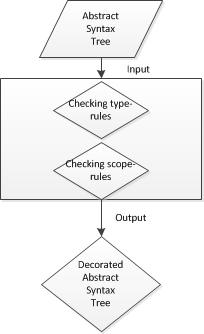
\includegraphics[scale=1]{rapport/6/figures/contextual_analyzer}
\label{fig:contextual_analyzer}
\caption{Contextual Analyzer}
\end{figure}

\begin{figure}[H]
\centering
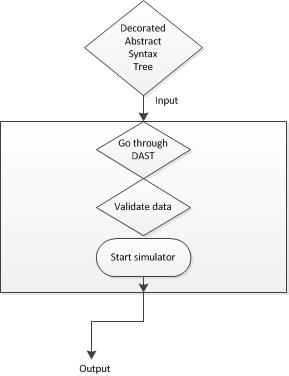
\includegraphics[scale=1]{rapport/6/figures/simulator}
\label{fig:simulator}
\caption{Simulator}
\end{figure}


\subsection{Simulation}

After getting the data and validating it, we are now able to start the simulator with the required data. 
The simulator reads and modifies a \textit{GameState} in every iteration or turn of the game. The \textit{GameState} contains the present formation of the game, where all the units are and how large the grid size is. In every iteration the interpreter updates the \textit{GameState}, the interpreter computes the \textit{Behaviour} from the teamfile.war script. Everytime a unit comes close to another unit and attacks, the interpreter computes how much damage is made, and in the end picks a winner. The output to the screen is made simple, and with the help of the Microsoft XNA \cite{XNA} Framework we have a simple simulation that can show several regiments behave differently and attacking each other.

%Pseudo-code for the algoritm
\subsubsection{Pseudo-code for the algorithm}
		\begin{lstlisting}[basicstyle=\small\sffamily,
		keywords={break,case,const,continue,default,else,enum,
		for,if,return,switch,while,do,long,void,int,float,double,
		char,struct,typedef,include,size\_t},
		keywordstyle={\color{blue}},
		comment={[l]{//}}, morecomment={[s]{/*}{*/}}, commentstyle=\itshape,
		columns={[l]flexible}, numbers=left, numberstyle=\tiny,
		frameround=fftt, frame=shadowbox, captionpos=b,
		caption={Team file},
		label=LST:code31]
While(Simulation == true)
{
	VisitorPattern(DAST); 		
	//Goes through the tree to gather data
	if(ValidateTheInput(DAST))	
	//Validates the data if there is anything missing
	{
		if(!GameState)			
		//Is this is the first iteration
		{
			CreateGameState(); 	
			//Creates a new GameState
		}
		ComputTheNextStep(BehaviourFromTeamfiles); 	
		//Next iteration, and computes the behaviour
		UpdateGameState();		
		//Updates a new GameState
		if (AnyWinner){Simulation = false}	
		//Checks for the winner, if any stop the simulation
	}
}
	\end{lstlisting}


%Pseudo-code done



%Interpreter eksekver en behaviour





